\documentclass[10pt]{article}
\usepackage[margin=0.65in]{geometry}
\usepackage{graphicx}
\usepackage[T1]{fontenc}
\usepackage{lmodern}
\begin{document}
\section*{N83 r29 fixed factor bases and model diagnostic}
The fixed-base enumeration covered 134,217,728 candidate x-coordinates for
each of the Koblitz, general binary, and prime families. It retained
134,195,671, 134,226,535, and 134,206,522 affine points, respectively, and
reused each exact base for m=2 through 9. The 384 payload/receipt shard pairs
cover contiguous selector ranges; the local index validation and all 48 PDP
input membership checks passed.

The exploratory seven-base training set has 336 matched rows. Its target is
the midpoint of a finite top-form degree interval, not exact degree of
regularity, FFD, or LFD. The grouped leave-one-base-out ridge fit has aggregate
MAE 2.5022 against 0.0000 for a matched-configuration baseline and wins zero
of seven held-out bases. All 48 matched top-form outcomes are identical across
the bases, so this fit finds no elite-base lead.

The diagnostic identifies a sampling limitation: planted tuples use common
support in the low 26 coordinates, and all seven bases repeat the same point
tuples in these PDP inputs. A lead-generating follow-up must sample
base-specific targets across the full 134-million-selector domain while retaining
the present common-support panel as a control. This is a post-label diagnostic
and does not establish a general base-quality result.

\begin{center}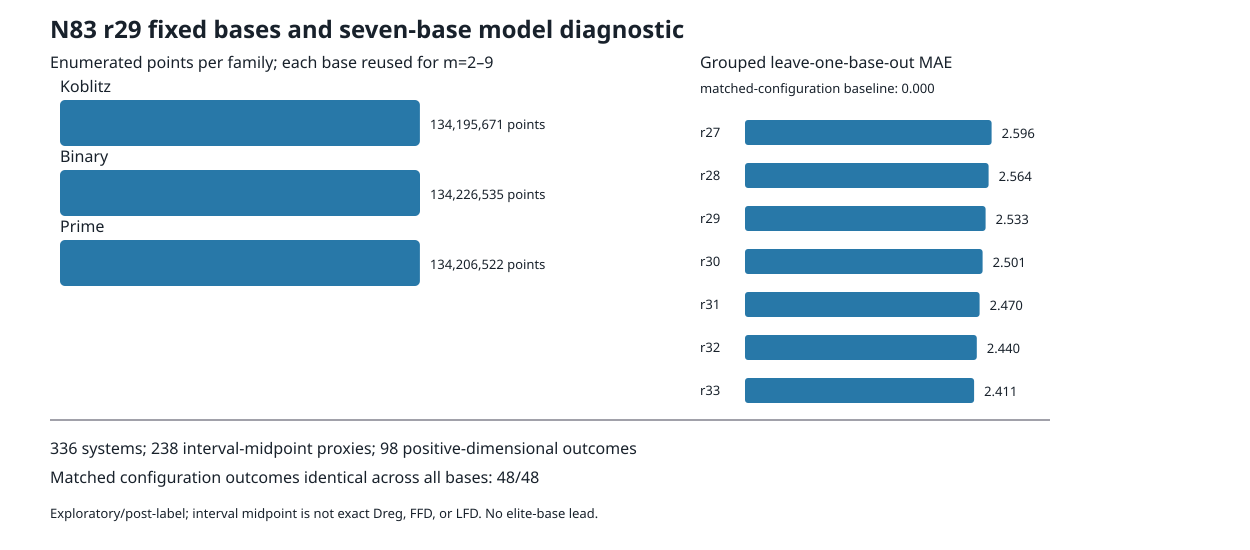
\includegraphics[width=\textwidth]{r29-model-diagnostic.png}\end{center}
\noindent Source files: factor-base index summary SHA-256
\texttt{f6787fb737fb988bcd5089fb1cb755b81f8745a7016e93d37d7c15bf87874236};
model protocol SHA-256
\texttt{2141d9f99a8bc07641b63db1a89d8f7fcaae9d29b4dfee6607e76592ec38e114}.
\end{document}
